\documentclass{llncs}
\usepackage[show]{ed}
\usepackage{calbf}
\usepackage{amstext,amsmath,amssymb}
\usepackage{xspace}

\usepackage{mdframed}
\newenvironment{boxedquote}{\begin{mdframed}[leftmargin=1cm,rightmargin=1cm]}{\end{mdframed}}

\usepackage{wrapfig,paralist}
\usepackage[hyperref,style=alphabetic]{biblatex}
\addbibresource{kwarcpubs.bib}
\addbibresource{extpubs.bib}
\addbibresource{kwarccrossrefs.bib}
\addbibresource{extcrossrefs.bib}
\addbibresource{rest.bib}

\pagestyle{plain}
\usepackage{tikz}\usetikzlibrary{docicon}

\usepackage{hyperref}
\title{System Description: A Semantics-Aware {\LaTeX}-to-WORD/ODF Converter}
\author{Lukas Kohlhase and Michael Kohlhase}
\institute{Mathematics/Computer Science\\
  Jacobs University Bremen}
\begin{document}
\maketitle
\begin{abstract}
  We present a {\LaTeX}-to-Office conversion plugin for {\LaTeX}ML that can bridge the
  divide between publication practices in the theoretical disciplines (\LaTeX) and the
  applied ones (predominantly Office). 
\end{abstract}

\section{Problem \& State of the Art}\label{sec:intro}

Many researchers in STEM fields only use {\LaTeX} to typeset their documents. However many
people still use Microsoft Word/Open office exclusively for their typesetting. When these
two groups of people intersect, it can lead to friction, as transforming text to {\LaTeX}
is quite trivial but not the opposite. For example if a conference requested documents in
Word format, the only recourse is often to just write the document in Word, which is a
pain, especially if any Mathematics is to be included.

\ednote{Here we state the Problem, some conferences and admin want papers in word format,
  however LaTeX is superior for various reasons. Hence converter is needed. Two step
  process, wastes some time.}

\begin{figure}[ht]
  \begin{tabular}{|c|c|}\hline%|
    copy from PDF & paste (libreoffice)\\\hline
    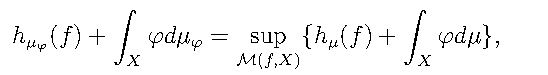
\includegraphics[width=6cm]{mathsnippet} & 
    
\includegraphics[width=5cm]{mathsnippet-libreoffice}\\\hline
  \end{tabular}
\caption{Copy \& Paste in Word Processors}\label{fig:cnp}
\end{figure}

There are several methods to transform papers from {\LaTeX} to an office word
processor. The first method is to just generate a PDF file and then open this file in
Word/LibreOffice. This achieves the goal of looking like the desired PDF document, just in
Office. There are two problems with this route: 
\begin{enumerate}
\item mathematical formulae are not preserved (see Figure~\ref{fig:cnp})
\item even if the result looks OK the results have lost their links (e.g. for
  citations/references or label/ref), or become difficult to edit, because they do not
  conform to the styling system of the word processor.
\end{enumerate}
The fundamental problem is that it converts the appearance of the document and loses
meaning due to macro expansion. This is especially blatant when looking at the math in a
document. Either it is treated as text, with no meaningful way to distinguish between math
and formatted text that happens to contain some mathematical symbols, making automatic
treatment of this kind of math difficult, or it is represented by an image of the relevant
formulae, which makes editing extremely impractical if not impossible. The same holds true
for references, they are essentially treated as parts of text with a linked number in
front of them, complicating adding new references substantially.

The other way of transforming {\LaTeX} to Word, by transforming the .tex file directly,
does away with some of these issues. Some editors to do this already exist, such as
TeX4ht~\cite{tex4ht:online}. This already does this admirably, however it is very focussed
on Libreoffice, e.g. it can't handle mathematics in docx files.

\section{Implementation}\label{sec:impl}

\begin{figure}[ht]\centering
\begin{tikzpicture}[yscale=1.5,xscale=1.2]
\tikzstyle{doc}=[draw,thick,align=center,color=black,
                 shape=document,minimum width=10mm,minimum height=8mm]
\node[doc] (p) at (-1,3.5) {\texttt{paper.tex}};
\node[doc] (b) at (1,3.5) {\texttt{group.bib}};
\node[doc,dashed] (px) at (-1,2.2) {\texttt{paper.ltxml}};
\node[doc,dashed] (bx) at (1,2.67) {\texttt{group.ltxml}};
\draw[->,thick] (p) -- node[left,near end] (l) {{\LaTeX}ML} (px);
\draw[->,thick] (b) -- (bx);
\draw[->,thick] (bx) -- (l);
\node[doc,dashed] (d) at (-2,1) {\texttt{document.xml}};
\node[doc,dashed] (r) at (0.2,1) {\texttt{relations.xml}};
\node[doc] (s) at (1,.3) {\texttt{styles.xml}};
\draw[->,thick] (px) -- node[left]{XSLT}(d);
\draw[->,thick] (px) -- node[right]{XSLT}(r); 
\node[inner sep=0pt,outer sep=0pt] (z) at (-1,.3) {};
\draw[thick] (d) -- (z);
\draw[thick] (r) -- (z);
\draw[thick] (s) -- (z);
\node[doc] (dx) at (0-1,-.4) {\texttt{paper.docx}};
\draw[->,thick] (z) -- node[left] {zip} (dx);
\draw[dotted] (-3.1,-.1) rectangle (1.9,1.9);
\node at (1.6,1.8) {post};
\end{tikzpicture}
\caption{The Transformation Process}\label{fig:arch}
\end{figure}

Both docx and odt files share a very similar structure and are almost interchangeable,
except for slight differences in syntax and different names. At heart they are both zipped
collections of XML files featuring one central document file and several supporting files
such as styles, settings etc. 

To create the .odt/.docx files we first transform the .tex file to an intermediate
XML-based format using {\LaTeX}ML. \ednote{Papa Latexml erlaerung einfuegen}.

Then we use XSLT stylesheets to semantically transform them to the required XML formats
and finally zip it using the {\LaTeX}ML post-processor. 

\ednote{Screenshot einfuegen}
\ednote{Bin eigentlich nicht zufrieden hiermit TT}

\section{Conclusion}\label{sec:concl}
In Conclusion we use {\LaTeX}ML and XSLT to transform {\LaTeX} files to Word/Office files
semantically in an easy to use process.  \ednote{In Conclusion, easy to use}

The {\LaTeX}ML Word Processing plugin is public domain and is available from GitHub
at~\cite{LaTeX2Office:github:on}

\printbibliography
\end{document}



%  LocalWords:  maketitle ednote hline libreoffice includegraphics mathsnippet cnp Hier
%  LocalWords:  einen einfuegen glaube ich docx impl odt Latexml erlaerung eigentlich
%  LocalWords:  nicht zufrieden hiermit concl printbibliography
